\section{Technical Development}
\subsection{User Interface Design}
The User interface for this project is designed after looking at the user interfaces used by other music applications. In particular, the developer was inspired by Spotify, shown in figure \ref{fig:spotify}.

\begin{figure}[h]
    \centering
    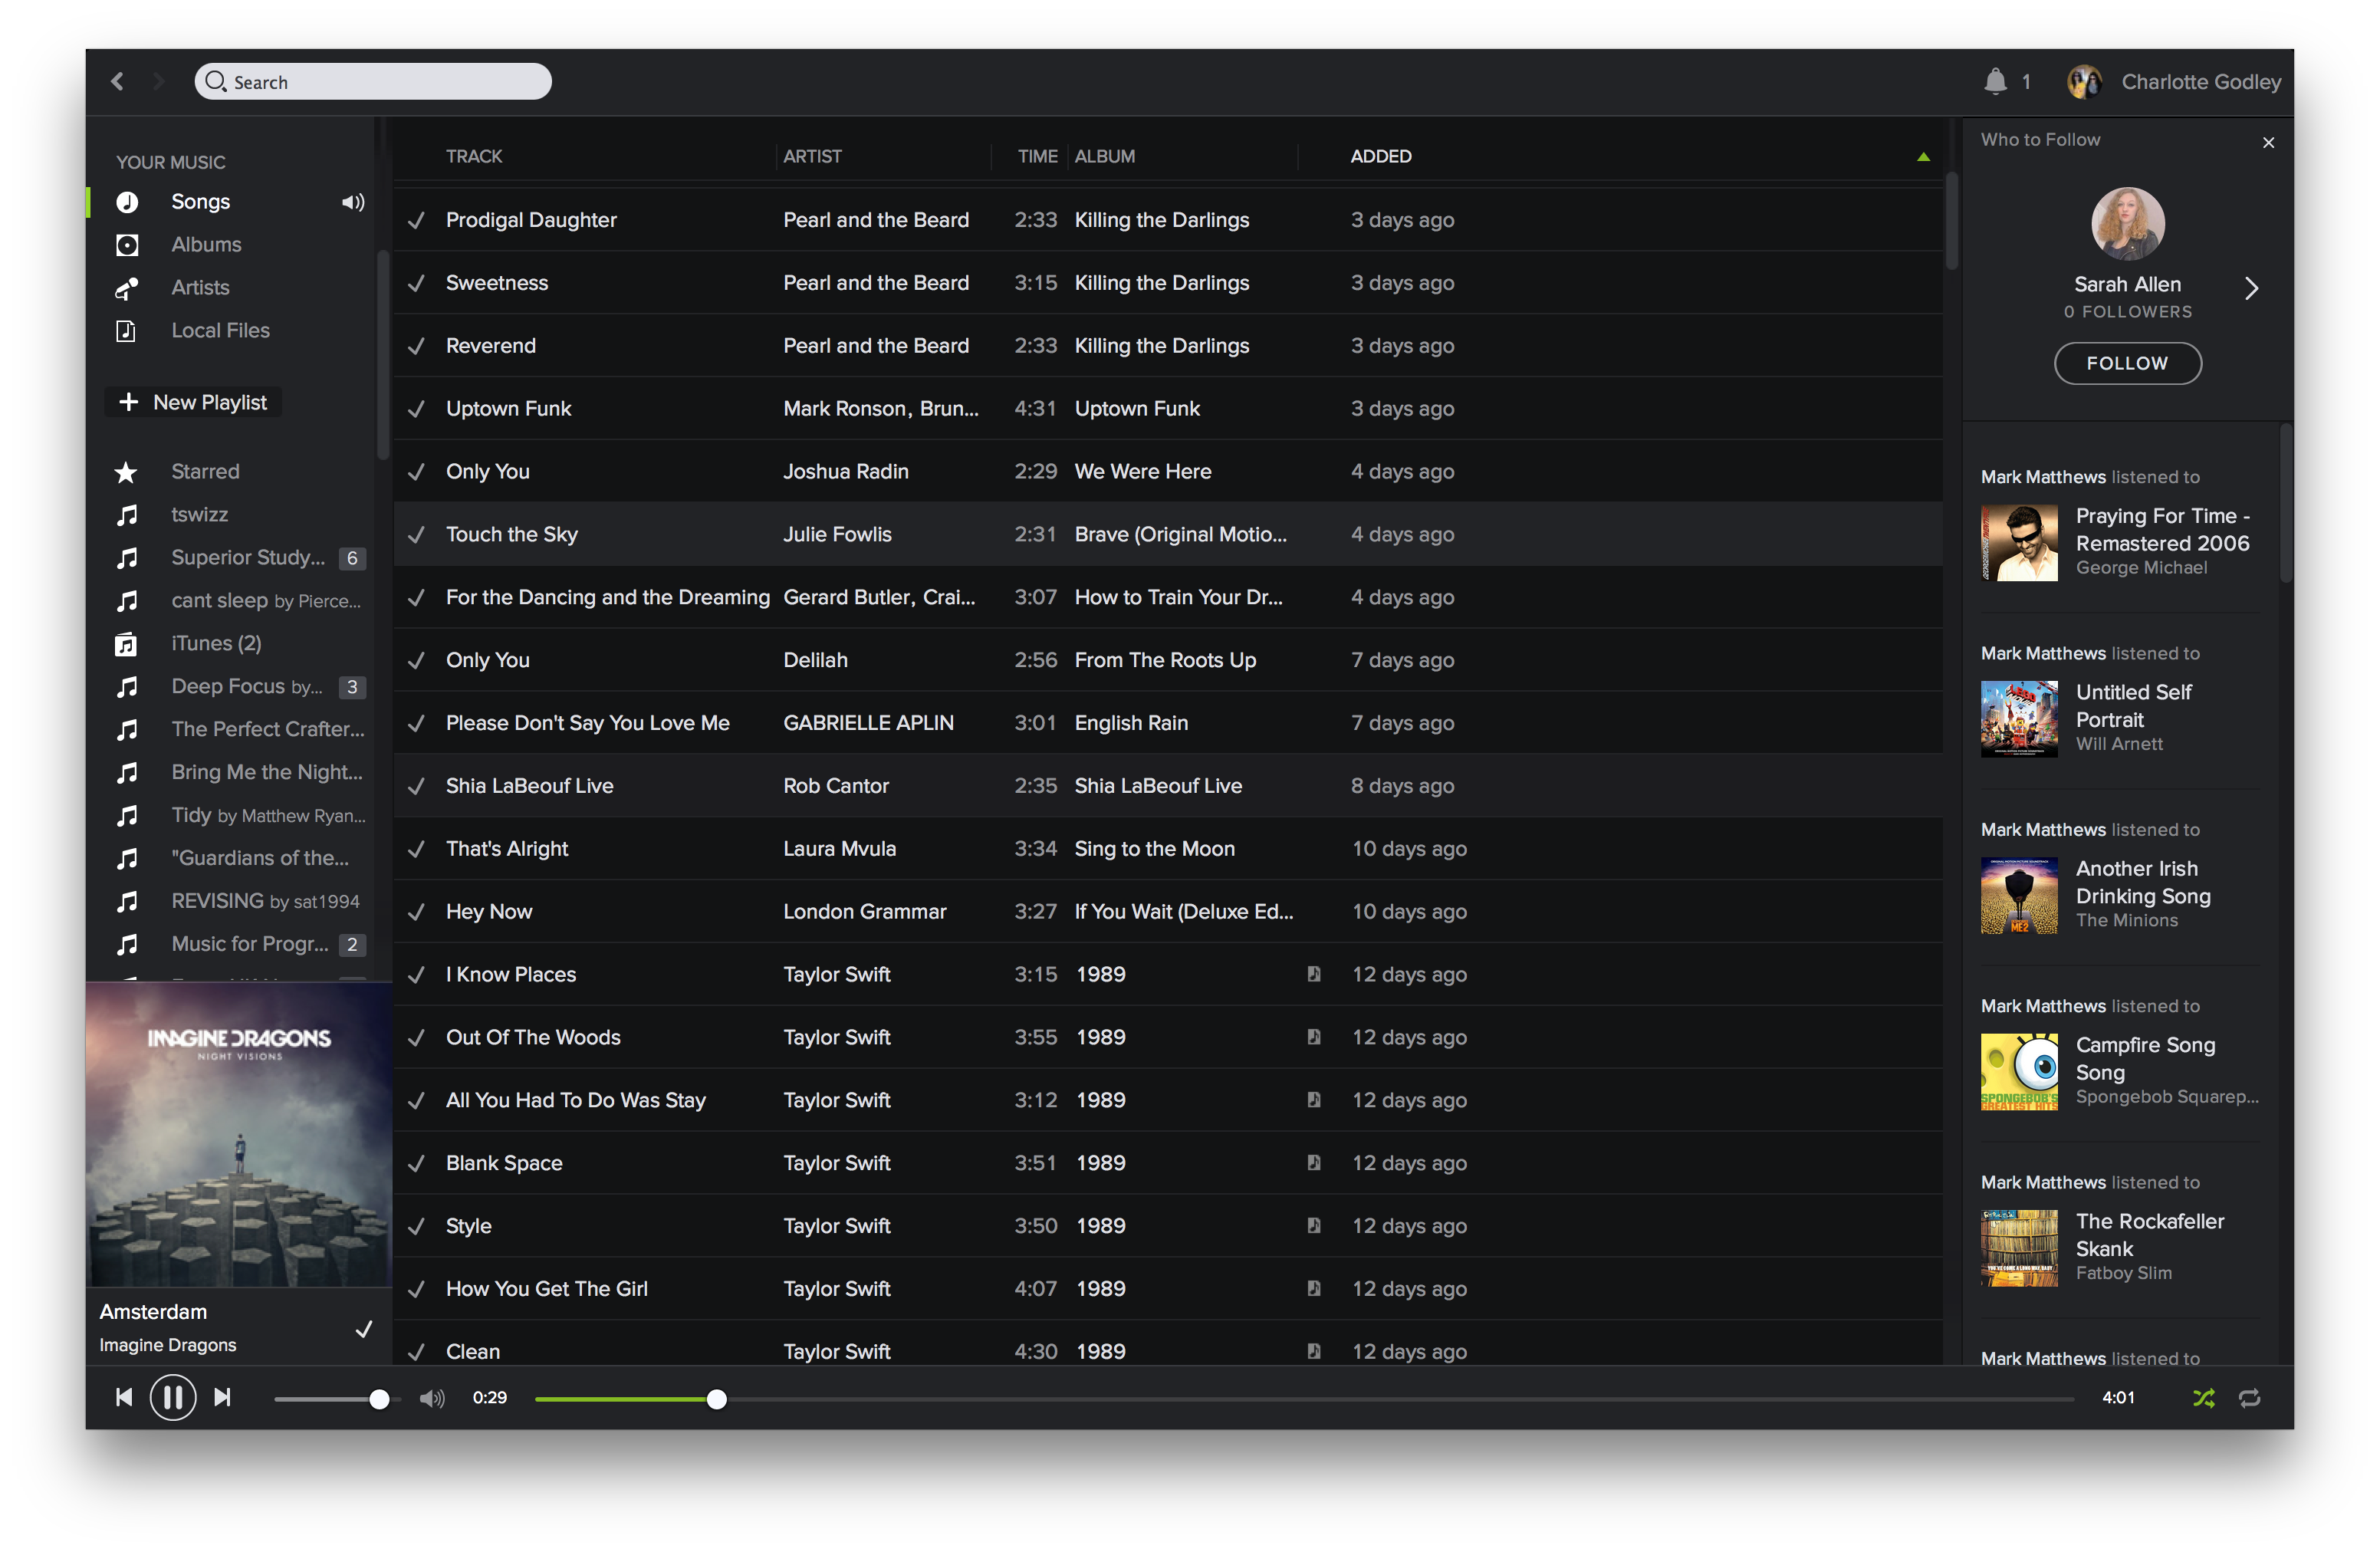
\includegraphics[width=\textwidth]{screen.png}
    \caption{Spotify user interface}
    \label{fig:spotify}
\end{figure}
\subsubsection{Main Display}
\begin{figure}[H]
    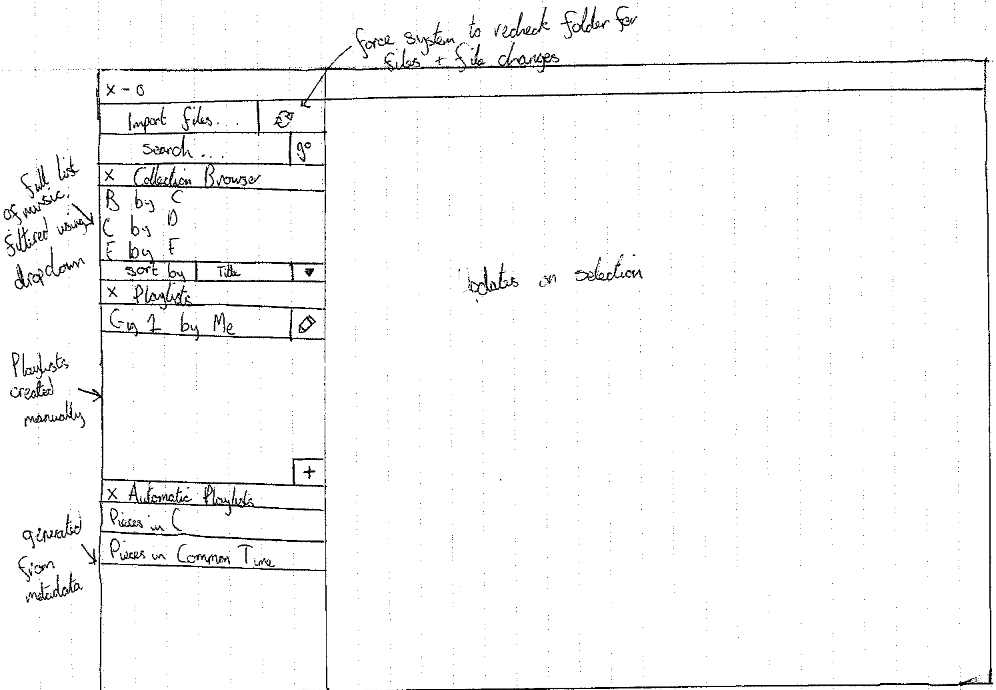
\includegraphics[width=400pt]{designs/main}
    \caption{Main User interface of the project}
    \label{fig:main}
\end{figure}
Figure \ref{fig:main} shows the main view of the application. Various panes to the left can be closed using the X button and show different ways the music can be displayed, either as individual units or as playlists. The larger pane next to it shows the area in which sheet music or a list of pieces in a playlist will be displayed, depending on the selection from the left pane. Updates to this and pop up boxes displaying dependent on buttons in the window are displayed and explained in the appendices.
\subsubsection{Musician feedback survey}
In order to understand how well this user interface works with a variety of users, a survey was designed which will be given to a selection of musicians, who will feedback on how easy the UI is to use and any updates which should be made to improve it. This feedback session will be performed after the initial sketches are made into a virtual user interface with no back end connected to the buttons. An example survey is provided in the appendices.
\subsection{Test Design and System Testing}
This project was developed using Test Driven Development. This is an Agile software development methodology which utilises the rules that a line of code should not be written unless there is a failing automated test \parencite{TDD}. This methodology has been chosen as the nature of the notation of music means that meticulous detail must be payed to how and with what symbol every element is notated, and Test Driven Development will significantly improve the quality of the software by closely integrating testing with the development process.

As such, no test design or plan was produced, but rather tests were developed as features were introduced, and were designed to be self contained units testing the smallest possible details, such as an accent being added to a measure correctly, or a note's pitch being created with a particular note name or octave number.

Test cases were created using the aforementioned software MuseScore. These were produced by creating a file for every area of notation (e.g. clefs, time signatures, note durations, pitch) and applying each and every symbol possible within that area to the music. It was decided to create test cases in this way to thoroughly ensure that no piece of notation was missed. An example testcase, and a list of all testcases in use and their value in real world testing, are included in the appendices.
Further to the testcases developed specifically for this application, the system was tested against a larger set of tests called "The Unofficial MusicXML testsuite", which was released by the Lilypond Project to provide a comprehensive test suite for all elements of MusicXML\parencite{LilypondTestcase}. 
Whilst the project was tested against all 131 files in the suite, around 65\% of these files passed, and the other 35\% which tested more specific notation were ignored in order to make way for other functionality. This decision was taken because the renderer took a long time to produce and continuing to ensure all of the tests passed would take time away from other more important features, and the elements which failed were minor. Despite their output not being perfect, the developer ensured that any failed testcases did not cause a system crash, and documented the problems using an issue tracker.
\subsection{System Design}
The class diagram in figure \ref{fig:classdiagram} shows an abstract structure of the renderer implementation used in this project. This implements a tree, each node of which holds an item defined at run time. Each item object and node object implements the ToLily method which outputs that node, node item and children's collateral lilypond-formatted string. A tree was chosen as the object structure in order to give an indication of time, and in order that specific elements could be positioned according to sequential instructions from the MusicXML parser. 
\begin{figure}[H]
    \centering
    \includegraphics[width=\textwidth]{diagrams/class_diagram_drawing}
    \caption{Renderer Class Diagram}
    \label{fig:classdiagram}
\end{figure}

The class diagram in figure \ref{fig:metadiagram} shows the structure of the meta and API portions of the system. This implements a layered structure as the MusicManager will be a member of the application layer, which handles input and manipulation of input from the main user interface. The music manager extracts and puts data into the data layer, which handles direct connections to and from the SQLite file where data will be stored.
\begin{figure}[H]
    \centering
    \includegraphics[width=\textwidth]{diagrams/api_and_meta_data_diagram}
    \caption{Metadata and API Class Diagram}
    \label{fig:metadiagram}
\end{figure}
The music manager class also handles connections to other classes, such as the folder browser, which handles scanning the folder for lists of xml and mxl files and compares them against a given list of files the music manager has in it's database, and the unzipper, which takes a list of mxl files, unzips and copies them into the relevant locations according to filename. 

Further to this, the API manager handles downloads of XML files for scanning, download of PDF files for viewing and collates data from all api sources so that the music manager can then choose what to do with this information, scan each downloaded file for metadata or allow the user to select a file for download. The dictionary stored in this manager can be extended to any number of apis which inherit from the API class, each indexed by the name of the API, which is then stored in the DataLayer when a new piece is downloaded and scanned from that API.


\subsection{System Implementation}
The project was implemented using a developer informed process, whereby the developer would review the project's status for bugs, issues and features which had yet to be implemented, note this using an issue tracker, develop unit tests for the issue and finally, develop the production code. Test Driven development, the portion of unit testing and production code creation, as previously mentioned was chosen as part of this development process in order to improve the quality and precision of the software. 


Issue tracking and reporting was used so that the developer could think and reflect on areas of the system which needed improvement, modification or implementation, and worked well in the context of a year long project in which development was not continuous because it ensured that when development was paused, the developer could see instantly what needed to be doing or what was being worked on before the pause to work on something else. This adds the benefit that in the future, when this project may be worked upon by more than one developer, new developers can see things which have yet to be implemented and choose which features are most relevant or doable by their own standards, as well as discuss or contest previous issues in the system.


The meta model for this project, which is arguably the focus of the project, was chosen because of personal preference as well as input from other musicians and research into what and how people categorise music. Upon research and creation of the project there was seemingly no standard meta model(ref). This is potentially due to the multi disciplinary problem, in which one model for music may not be relevant to another research project due to the design and implementation aims of that project, and therefore researchers may not think it relevant or necessary to publish the model for their project\parencite{MIR}. For example, a musicology project analysing chord patterns of 18th century music would have very different goals to a music technology project aiming to improve the electronic synthesis of classical music. It is hoped that publishing and open sourcing this project will make way for a standard model, as the model used in this project is intended to be broad enough to apply to most implementations. 

It should also be noted that whilst the initial objective of this project was to render sheet music from XML, there does not appear to be a standard implementation for how this should be done either, with different projects choosing their own class structures depending on their area\parencite{Music21}. This is potentially due to lack of interest in digitising or automating the process, lack of knowledge of the standard file format for knowledgeable music or for some other reason. Nonetheless, it is hoped that the time spent developing a working renderer at the initial stage of this project, which took longer than expected and required in depth knowledge and understanding of both input and output formats, will help to standardise the rendering process for future research projects when the code is open sourced.


mention difficulty rating has not been done in other apps in particular, so research had to be done into how people rank music
